% --------------------------------------------------------------
% This is all preamble stuff that you don't have to worry about.
% Head down to where it says "Start here"
% --------------------------------------------------------------

\documentclass[12pt]{article}
 
\usepackage[margin=1in]{geometry}
\usepackage{amsmath,amsthm,amssymb}

\usepackage{listings}
\usepackage{xcolor}

\usepackage{tikz}
\usetikzlibrary{shapes,positioning}

\tikzset{ell/.style={ellipse,draw,minimum height=0.1cm,minimum width=0.1cm,inner sep=0.1cm}}

%New colors defined below
\definecolor{codegreen}{rgb}{0,0.6,0}
\definecolor{codegray}{rgb}{0.5,0.5,0.5}
\definecolor{codepurple}{rgb}{0.58,0,0.82}
\definecolor{backcolour}{rgb}{0.95,0.95,0.92}

%Code listing style named "mystyle"
\lstdefinestyle{mystyle}{
  backgroundcolor=\color{backcolour}, commentstyle=\color{codegreen},
  keywordstyle=\color{magenta},
  numberstyle=\tiny\color{codegray},
  stringstyle=\color{codepurple},
  basicstyle=\ttfamily\footnotesize,
  breakatwhitespace=false,         
  breaklines=true,                 
  captionpos=b,                    
  keepspaces=true,                 
  numbers=left,                    
  numbersep=5pt,                  
  showspaces=false,                
  showstringspaces=false,
  showtabs=false,                  
  tabsize=2
}

%"mystyle" code listing set
\lstset{style=mystyle}

\newcommand{\N}{\mathbb{N}}
\newcommand{\Z}{\mathbb{Z}}

\newenvironment{theorem}[2][Theorem]{\begin{trivlist}
\item[\hskip \labelsep {\bfseries #1}\hskip \labelsep {\bfseries #2.}]}{\end{trivlist}}
\newenvironment{lemma}[2][Lemma]{\begin{trivlist}
\item[\hskip \labelsep {\bfseries #1}\hskip \labelsep {\bfseries #2.}]}{\end{trivlist}}
\newenvironment{exercise}[2][Exercise]{\begin{trivlist}
\item[\hskip \labelsep {\bfseries #1}\hskip \labelsep {\bfseries #2.}]}{\end{trivlist}}
\newenvironment{problem}[2][Problem]{\begin{trivlist}
\item[\hskip \labelsep {\bfseries #1}\hskip \labelsep {\bfseries #2.}]}{\end{trivlist}}
\newenvironment{question}[2][Question]{\begin{trivlist}
\item[\hskip \labelsep {\bfseries #1}\hskip \labelsep {\bfseries #2.}]}{\end{trivlist}}
\newenvironment{corollary}[2][Corollary]{\begin{trivlist}
\item[\hskip \labelsep {\bfseries #1}\hskip \labelsep {\bfseries #2.}]}{\end{trivlist}}

\begin{document}

% --------------------------------------------------------------
%                         Start here
% --------------------------------------------------------------

\title{Teamwork 3}%replace X with the appropriate number
\author{Mengxiang Jiang\\ %replace with your name
CSEN 5303 Foundations of Computer Science} %if necessary, replace with your course title

\maketitle
\begin{problem}{(Decision Tree)}
    Consider a set of four distinct integers $a$, $b$, $c$, and $d$.
\begin{quote}
    1. Give the decision tree for insertion sort operating on integers $a$, $b$, $c$, and $d$.
\end{quote}
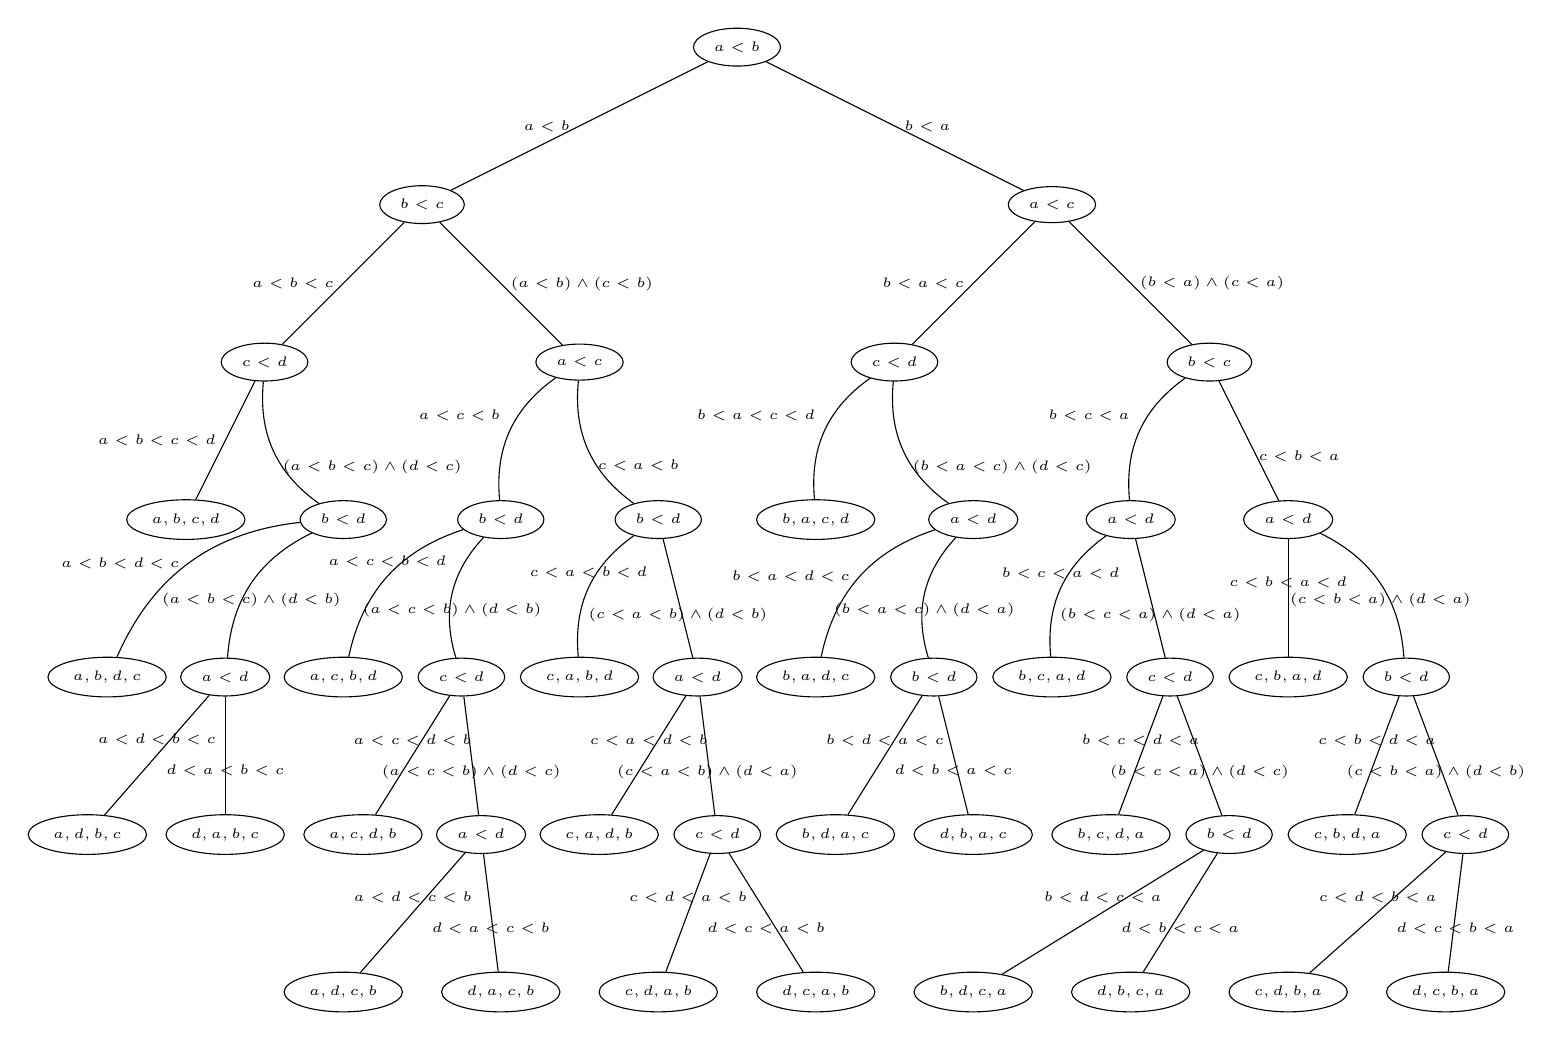
\begin{tikzpicture}[>=stealth]
    \node[ell] (a)at (8,6) {\tiny$a < b$};
    \node[ell] (b)at (4,4) {\tiny$b < c$};
    \node[ell] (c)at (12,4) {\tiny$a < c$};
    \node[ell] (d)at (2,2) {\tiny$c < d$};
    \node[ell] (e)at (6,2) {\tiny$a < c$};
    \node[ell] (f)at (10,2) {\tiny$c < d$};
    \node[ell] (g)at (14,2) {\tiny$b < c$};
    \node[ell] (h)at (1,0) {\tiny$a,b,c,d$};
    \node[ell] (i)at (3,0) {\tiny$b < d$};
    \node[ell] (j)at (5,0) {\tiny$b < d$};
    \node[ell] (k)at (7,0) {\tiny$b < d$};
    \node[ell] (l)at (9,0) {\tiny$b,a,c,d$};
    \node[ell] (m)at (11,0) {\tiny$a < d$};
    \node[ell] (n)at (13,0) {\tiny$a < d$};
    \node[ell] (o)at (15,0) {\tiny$a < d$};
    \node[ell] (p)at (0,-2) {\tiny$a,b,d,c$};
    \node[ell] (q)at (1.5,-2) {\tiny$a < d$};
    \node[ell] (r)at (3,-2) {\tiny$a,c,b,d$};
    \node[ell] (s)at (4.5,-2) {\tiny$c<d$};
    \node[ell] (t)at (6,-2) {\tiny$c,a,b,d$};
    \node[ell] (u)at (7.5,-2) {\tiny$a<d$};
    \node[ell] (v)at (9,-2) {\tiny$b,a,d,c$};
    \node[ell] (w)at (10.5,-2) {\tiny$b<d$};
    \node[ell] (x)at (12,-2) {\tiny$b,c,a,d$};
    \node[ell] (y)at (13.5,-2) {\tiny$c<d$};
    \node[ell] (z)at (15,-2) {\tiny$c,b,a,d$};
    \node[ell] (a2)at (16.5,-2) {\tiny$b<d$};
    \node[ell] (b2)at (-0.25,-4) {\tiny$a,d,b,c$};
    \node[ell] (c2)at (1.5,-4) {\tiny$d,a,b,c$};
    \node[ell] (d2)at (3.25,-4) {\tiny$a,c,d,b$};
    \node[ell] (e2)at (4.75,-4) {\tiny$a<d$};
    \node[ell] (f2)at (6.25,-4) {\tiny$c,a,d,b$};
    \node[ell] (g2)at (7.75,-4) {\tiny$c<d$};
    \node[ell] (h2)at (9.25,-4) {\tiny$b,d,a,c$};
    \node[ell] (i2)at (11,-4) {\tiny$d,b,a,c$};
    \node[ell] (j2)at (12.75,-4) {\tiny$b,c,d,a$};
    \node[ell] (k2)at (14.25,-4) {\tiny$b<d$};
    \node[ell] (l2)at (15.75,-4) {\tiny$c,b,d,a$};
    \node[ell] (m2)at (17.25,-4) {\tiny$c<d$};
    \node[ell] (n2)at (3,-6) {\tiny$a,d,c,b$};
    \node[ell] (o2)at (5,-6) {\tiny$d,a,c,b$};
    \node[ell] (p2)at (7,-6) {\tiny$c,d,a,b$};
    \node[ell] (q2)at (9,-6) {\tiny$d,c,a,b$};
    \node[ell] (r2)at (11,-6) {\tiny$b,d,c,a$};
    \node[ell] (s2)at (13,-6) {\tiny$d,b,c,a$};
    \node[ell] (t2)at (15,-6) {\tiny$c,d,b,a$};
    \node[ell] (u2)at (17,-6) {\tiny$d,c,b,a$};
  
    \draw [] (a) to []node[left]{\tiny$a < b$} (b);
    \draw [] (a) to []node[right]{\tiny$b < a$} (c);
    \draw [] (b) to []node[left]{\tiny$a < b < c$} (d);
    \draw [] (b) to []node[right]{\tiny$(a < b) \land (c < b)$} (e);
    \draw [] (c) to []node[left]{\tiny$b < a < c$} (f);
    \draw [] (c) to []node[right]{\tiny$(b < a) \land (c < a)$} (g);
    \draw [] (d) to []node[left]{\tiny$a<b<c<d$} (h);
    \draw [] (d) to [bend right]node[below right]{\tiny$(a<b<c)\land (d<c)$} (i);
    \draw [] (e) to [bend right]node[above left]{\tiny$a<c<b$} (j);
    \draw [] (e) to [bend right]node[below right]{\tiny$c<a<b$} (k);
    \draw [] (f) to [bend right]node[above left]{\tiny$b<a<c<d$} (l);
    \draw [] (f) to [bend right]node[below right]{\tiny$(b<a<c) \land (d<c)$} (m);
    \draw [] (g) to [bend right]node[above left]{\tiny$b<c<a$} (n);
    \draw [] (g) to []node[below right]{\tiny$c<b<a$} (o);
    \draw [] (i) to [bend right]node[left]{\tiny$a<b<d<c$} (p);
    \draw [] (i) to [bend right]node[below]{\tiny$(a<b<c) \land (d<b)$} (q);
    \draw [] (j) to [bend right]node[above]{\tiny$a<c<b<d$} (r);
    \draw [] (j) to [bend right]node[below]{\tiny$(a<c<b) \land (d<b)$} (s);
    \draw [] (k) to [bend right]node[above]{\tiny$c<a<b<d$} (t);
    \draw [] (k) to []node[below]{\tiny$(c<a<b) \land (d<b)$} (u);
    \draw [] (m) to [bend right]node[left]{\tiny$b<a<d<c$} (v);
    \draw [] (m) to [bend right]node[below]{\tiny$(b<a<c) \land (d<a)$} (w);
    \draw [] (n) to [bend right]node[above]{\tiny$b<c<a<d$} (x);
    \draw [] (n) to []node[below]{\tiny$(b<c<a) \land (d<a)$} (y);
    \draw [] (o) to []node[above]{\tiny$c<b<a<d$} (z);
    \draw [] (o) to [bend left]node[below]{\tiny$(c<b<a) \land (d<a)$} (a2);
    \draw [] (q) to []node[above]{\tiny$a<d<b<c$} (b2);
    \draw [] (q) to []node[below]{\tiny$d<a<b<c$} (c2);
    \draw [] (s) to []node[above]{\tiny$a<c<d<b$} (d2);
    \draw [] (s) to []node[below]{\tiny$(a<c<b)\land(d<c)$} (e2);
    \draw [] (u) to []node[above]{\tiny$c<a<d<b$} (f2);
    \draw [] (u) to []node[below]{\tiny$(c<a<b)\land(d<a)$} (g2);
    \draw [] (w) to []node[above]{\tiny$b<d<a<c$} (h2);
    \draw [] (w) to []node[below]{\tiny$d<b<a<c$} (i2);
    \draw [] (y) to []node[above]{\tiny$b<c<d<a$} (j2);
    \draw [] (y) to []node[below]{\tiny$(b<c<a)\land(d<c)$} (k2);
    \draw [] (a2) to []node[above]{\tiny$c<b<d<a$} (l2);
    \draw [] (a2) to []node[below]{\tiny$(c<b<a)\land(d<b)$} (m2);
    \draw [] (e2) to []node[above]{\tiny$a<d<c<b$} (n2);
    \draw [] (e2) to []node[below]{\tiny$d<a<c<b$} (o2);
    \draw [] (g2) to []node[above]{\tiny$c<d<a<b$} (p2);
    \draw [] (g2) to []node[below]{\tiny$d<c<a<b$} (q2);
    \draw [] (k2) to []node[above]{\tiny$b<d<c<a$} (r2);
    \draw [] (k2) to []node[below]{\tiny$d<b<c<a$} (s2);
    \draw [] (m2) to []node[above]{\tiny$c<d<b<a$} (t2);
    \draw [] (m2) to []node[below]{\tiny$d<c<b<a$} (u2);

  \end{tikzpicture}

\begin{quote}
    2. How many comparisons does your algorithm do in the worst case? On the average?
\end{quote}
The worst case number of comparisons is 6.\\
On average the number of comparisons is\\
$\frac{2*3 + 6*4 + 8*5 + 8*6}{24} = \frac{118}{24} = \frac{59}{12} \approx 4.9$.

\end{problem}
% --------------------------------------------------------------
%     You don't have to mess with anything below this line.
% --------------------------------------------------------------

\end{document}